
\begin{figure}[H]
    \centering
    \caption{Decisions by Coalition Type and Term (2018 to 2023 Terms)}
    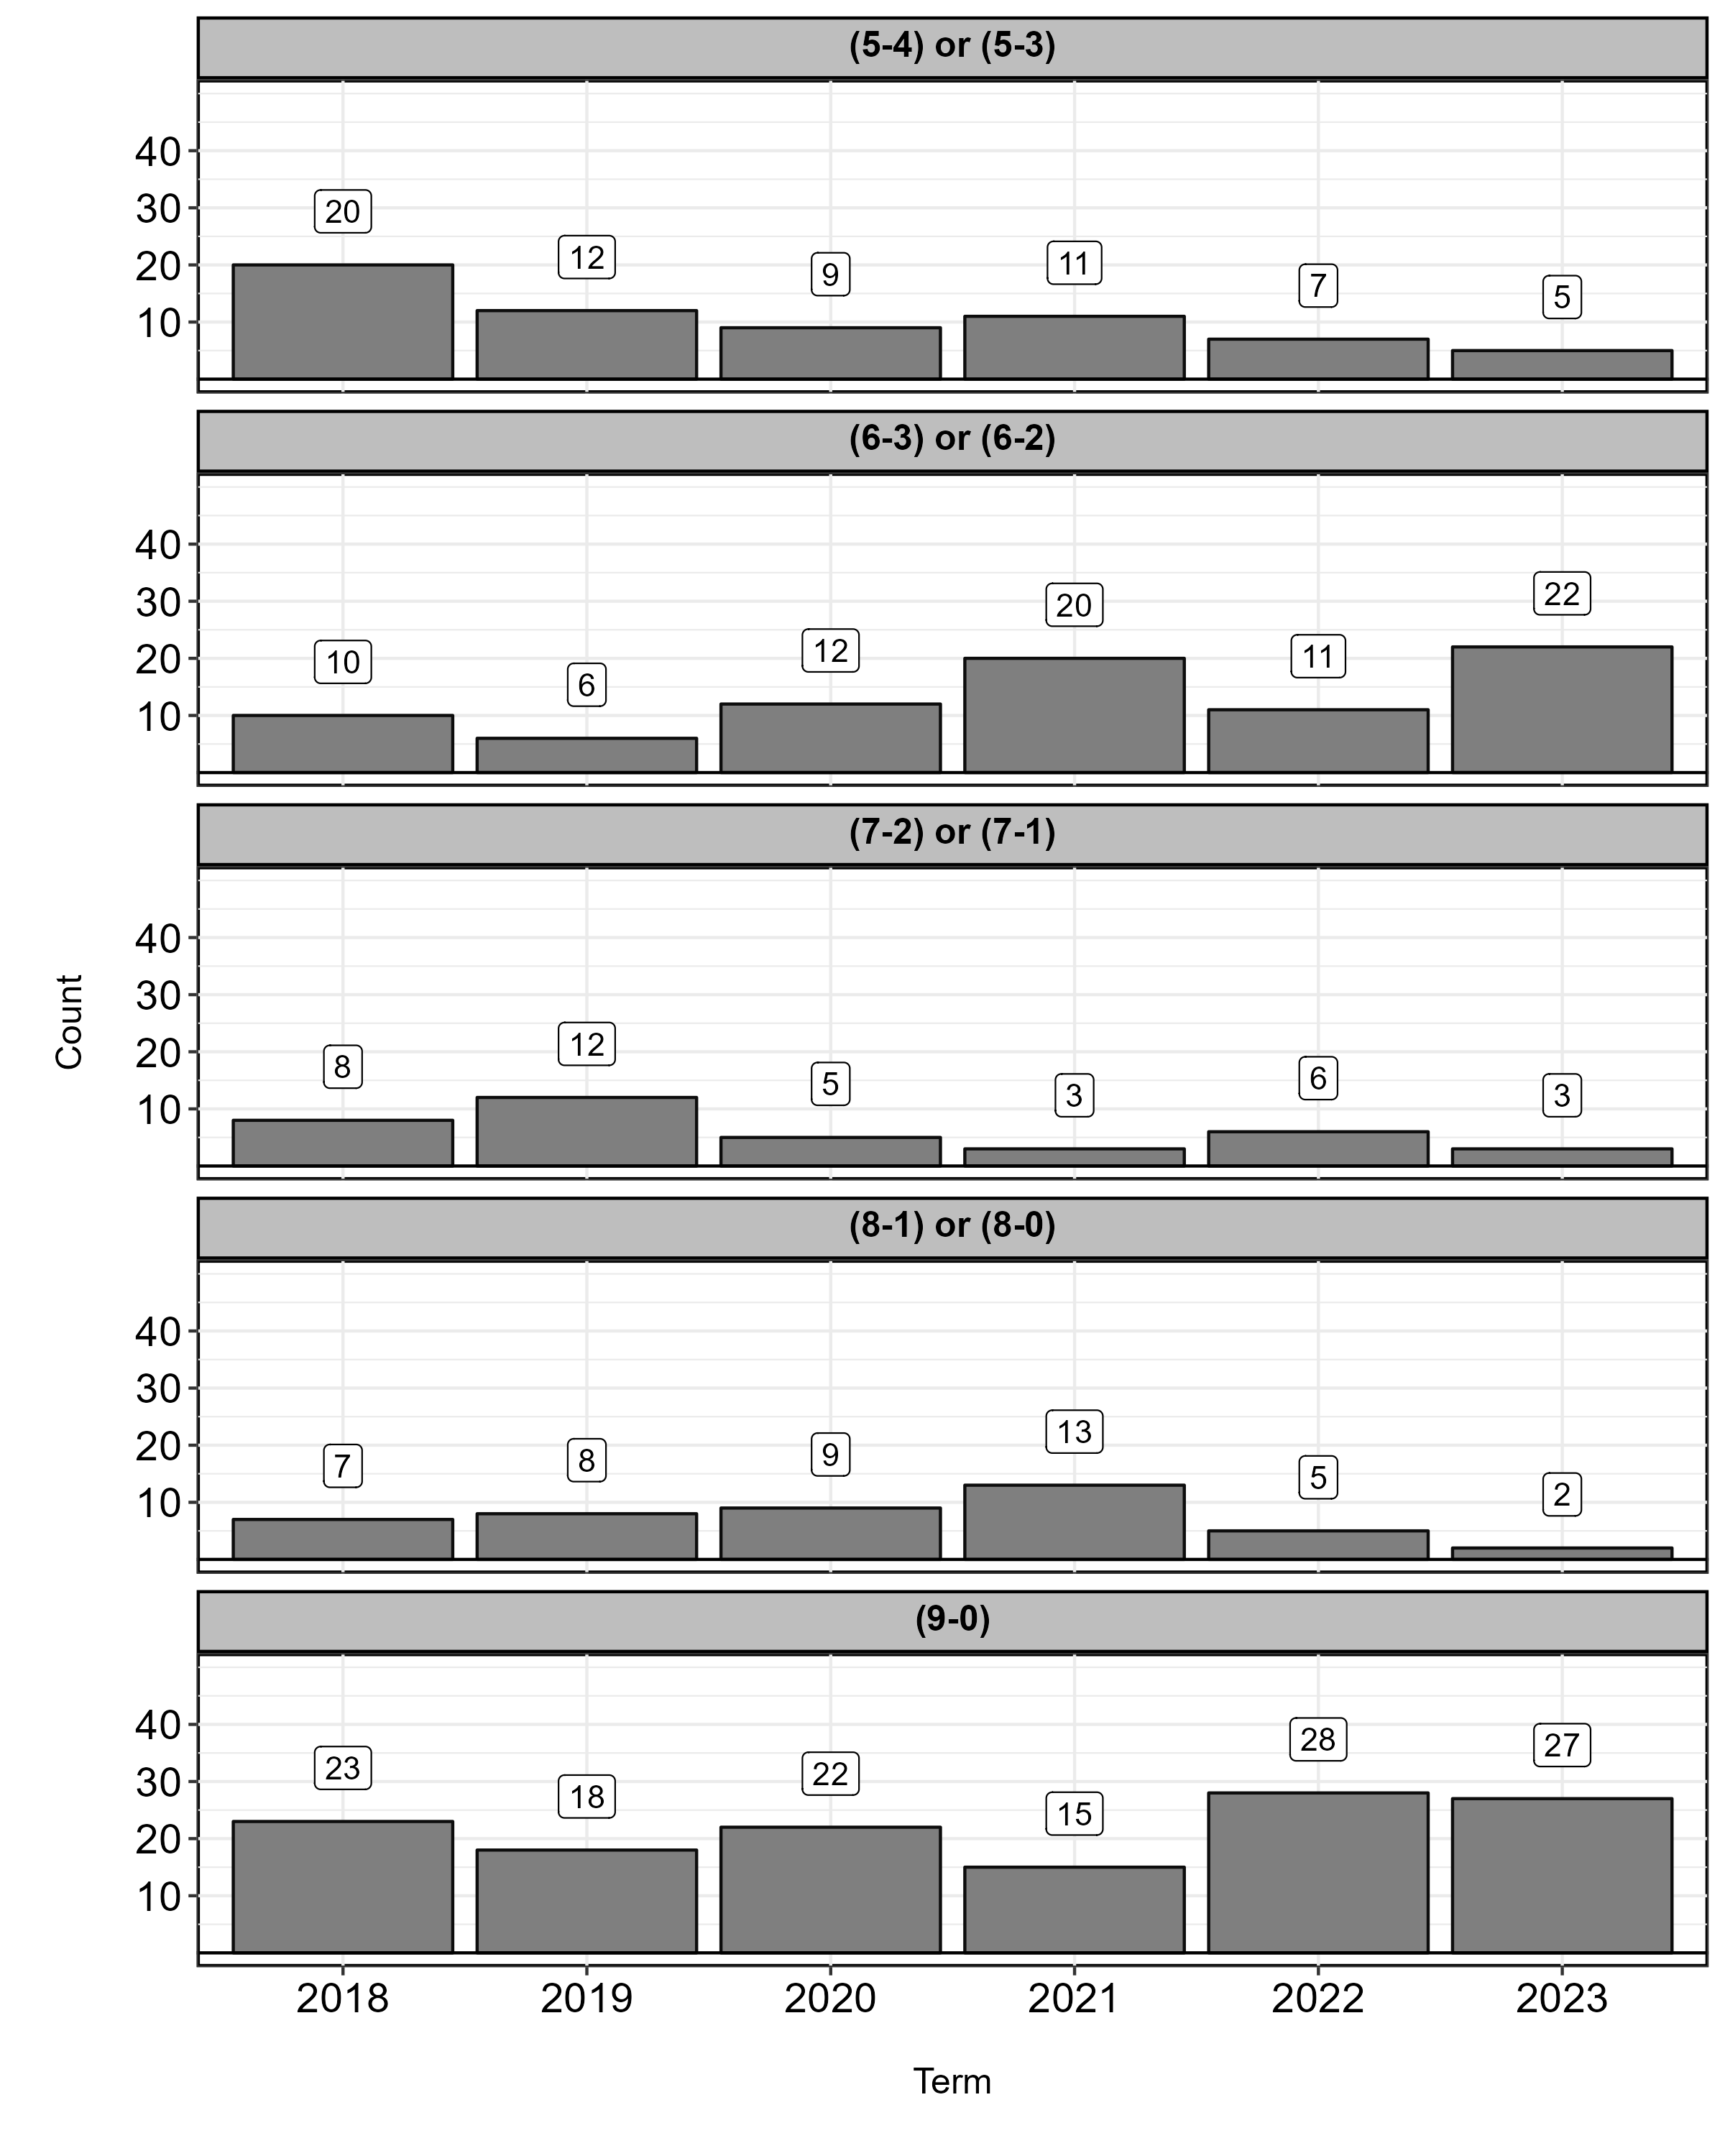
\includegraphics[width=0.9\textwidth]{Figures/statpack_figures/decisions_by_coalition_2018_2023.png} \\
    \footnotesize{Data Source: 2018 to 2022 Terms Compiled from Supreme Court Database (WUSTL)} \\
    \footnotesize{\emph{Note}: (9-0) does not consider whether concurrences (Regular, Special, or \emph{In Judgement}) were filed.}
\end{figure}


\begin{landscape}
\begin{figure}[H]
    \centering
    \caption{Share of Cases Decided Unanimously by Term}
    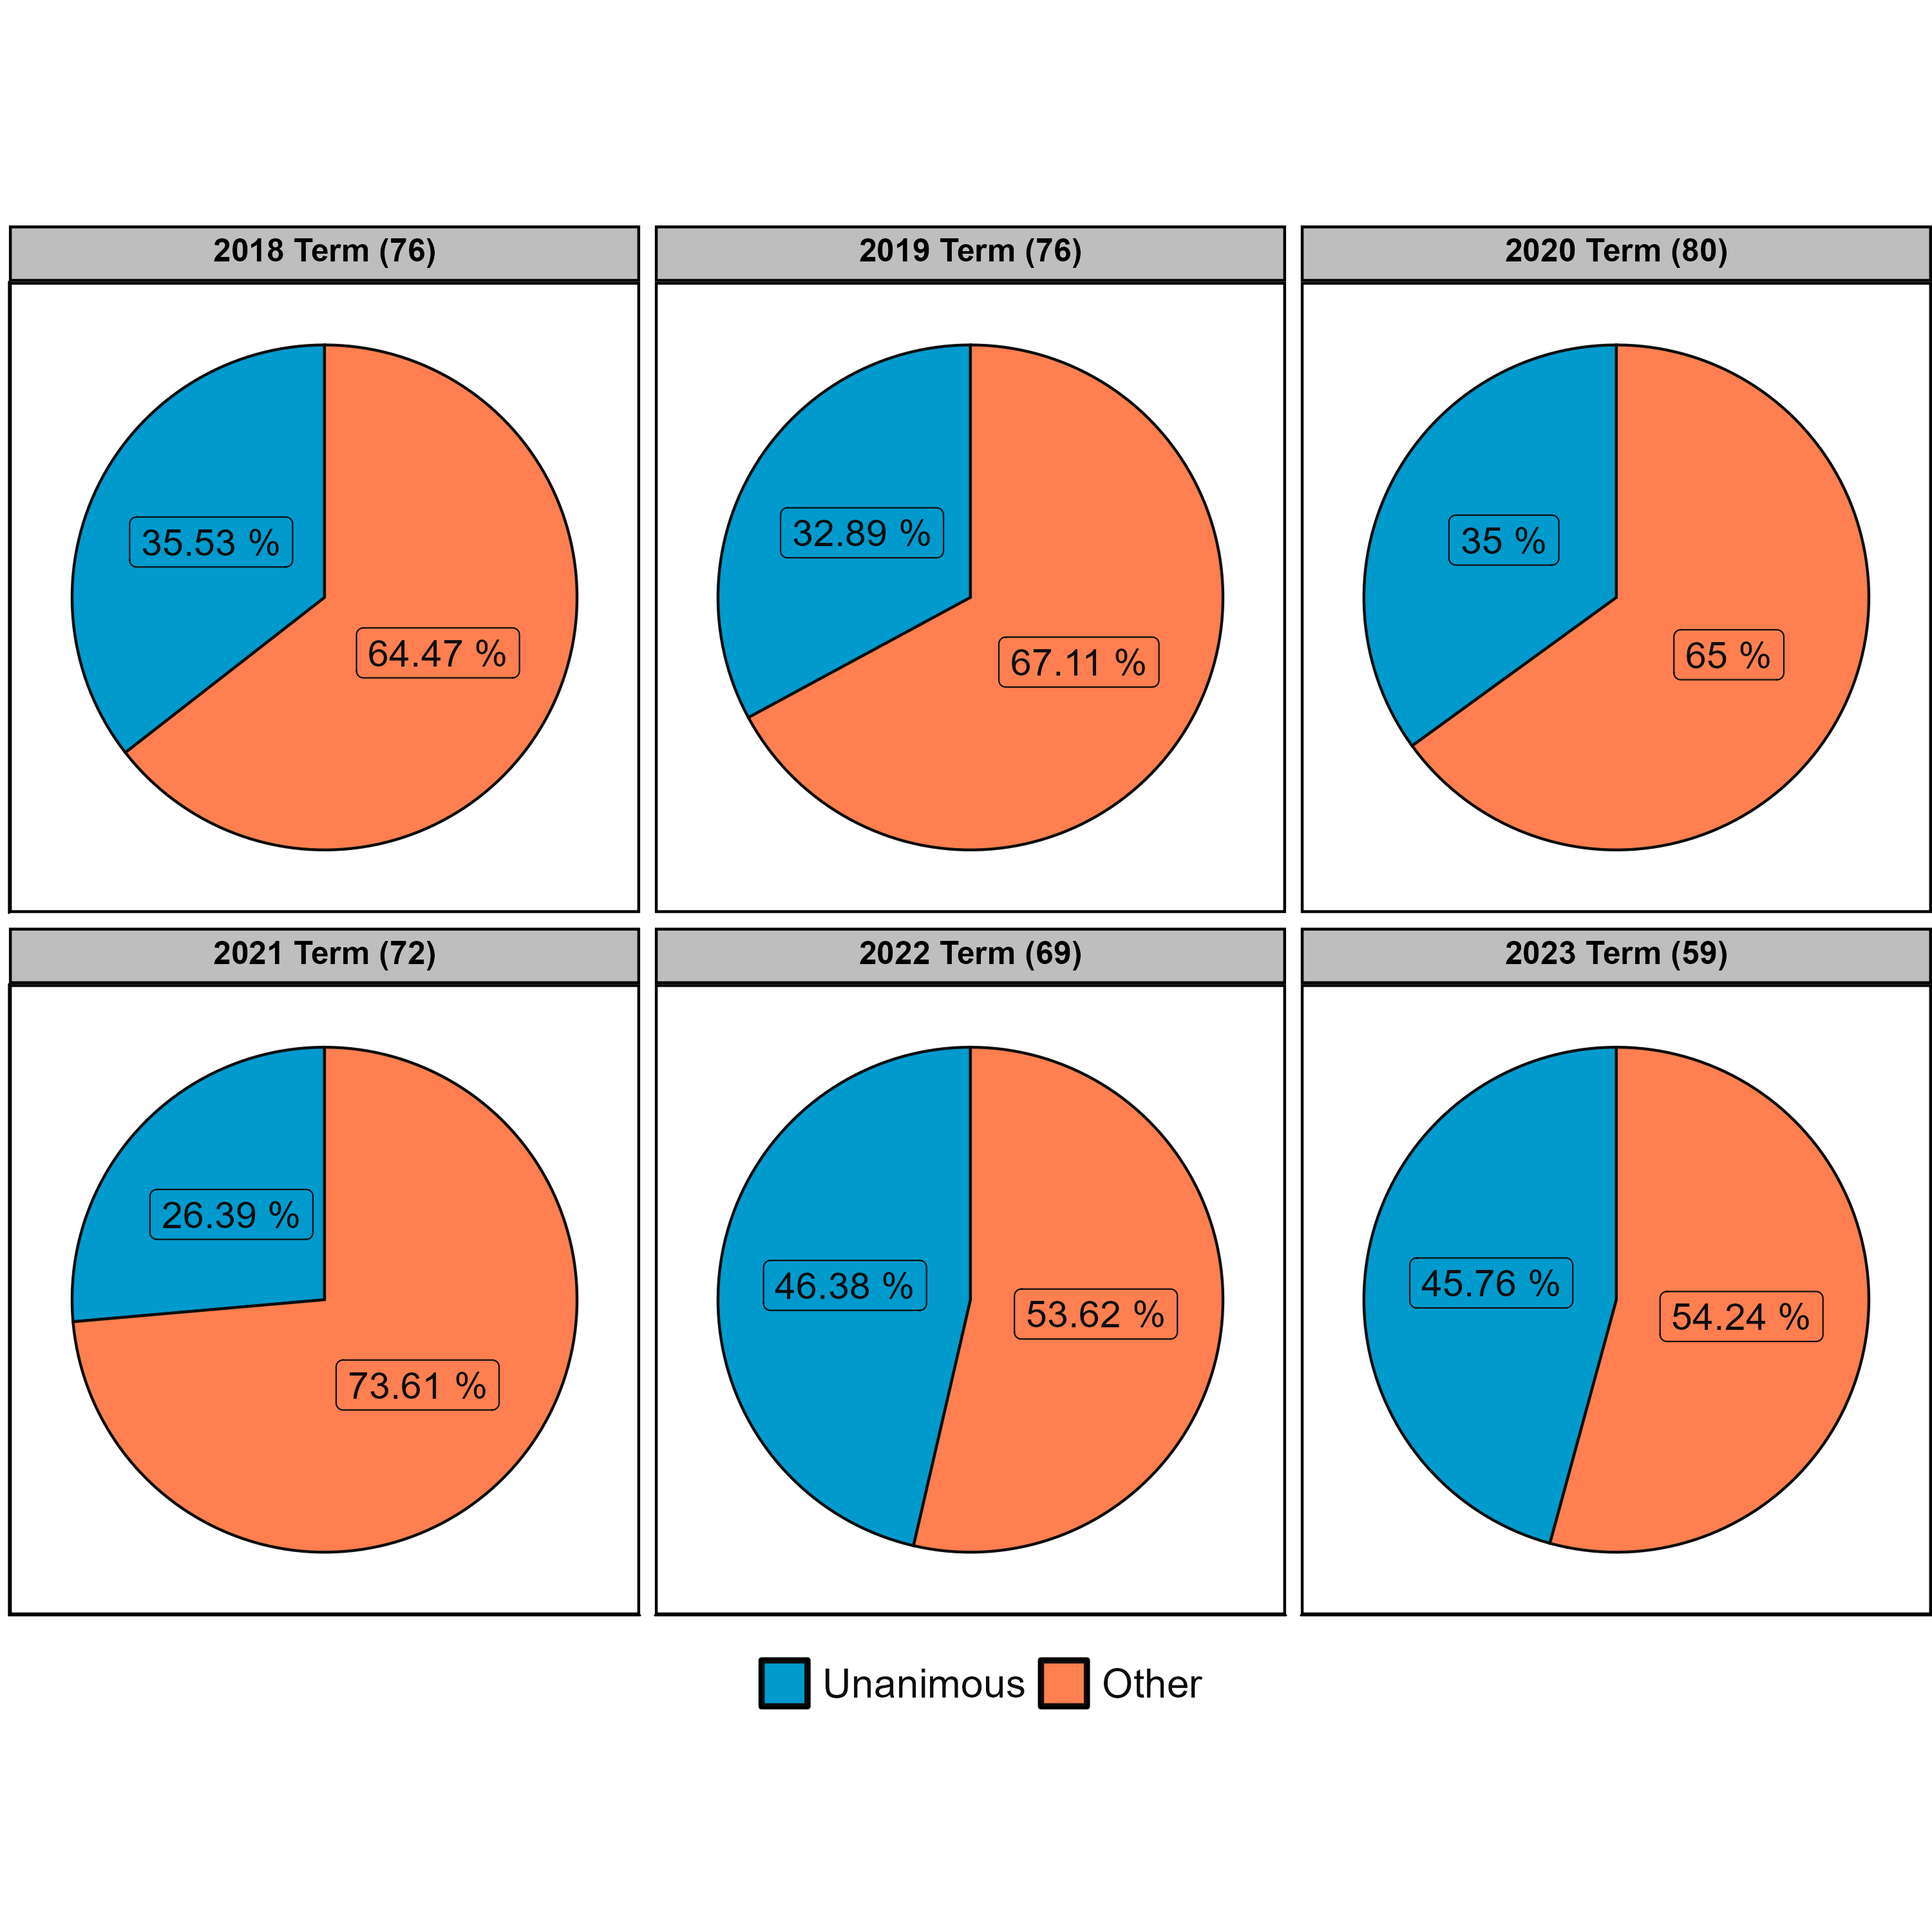
\includegraphics[width=0.8\textwidth]{Figures/statpack_figures/share_of_unanimity_2018_2023.png} \\
    \footnotesize{Data Source: 2018 to 2022 Terms Compiled from Supreme Court Database} \\
    \footnotesize{\emph{Note}: Unanimous (9-0 or 8-0) does not consider whether concurrences (Regular, Special, or \emph{In Judgement}) were filed.} \\
    \footnotesize{\emph{Note}: Parentheses beside term label represents total number of cases during term.}
\end{figure}
\end{landscape}


%\begin{landscape}
%\begin{figure}[H]
%    \centering
%    \caption{Share of Cases Where Dissent or Concurrence Filed}
%    \vspace{2.5mm}
%    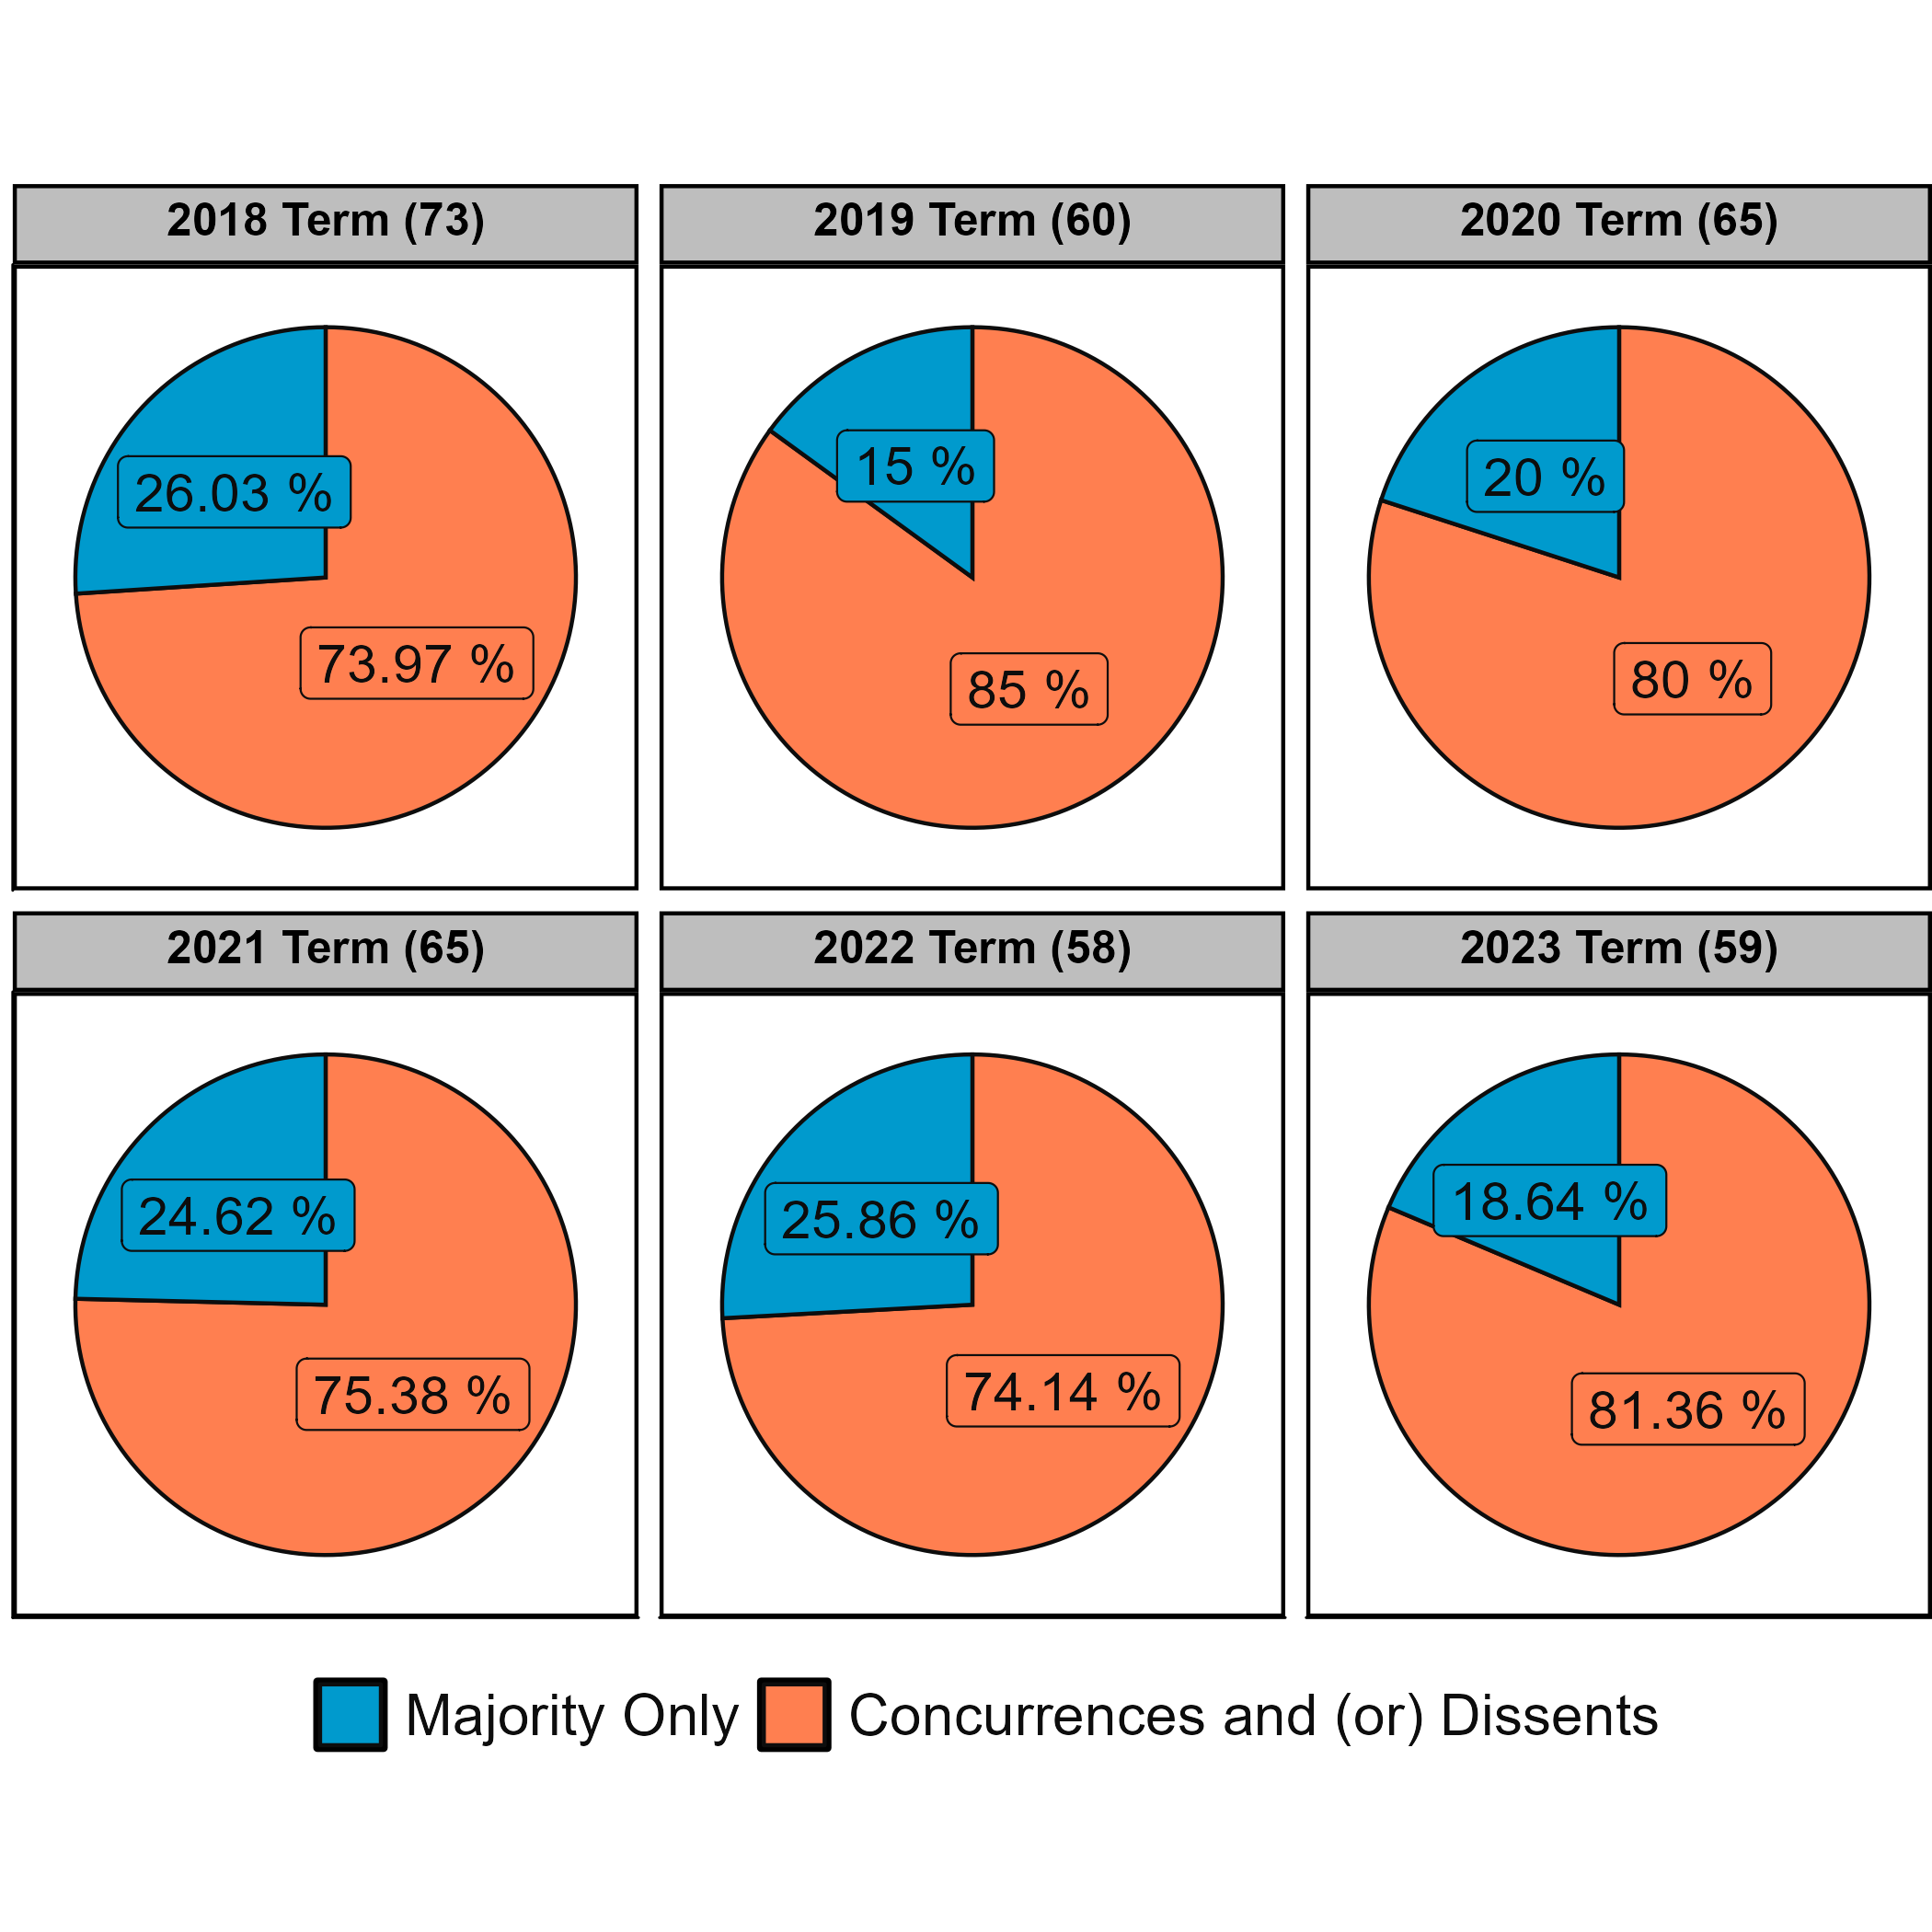
\includegraphics[width=0.8\textwidth]{Figures/statpack_figures/opinion_type_share_18_23.png} \\
%    \footnotesize{Data Source: 2018 to 2022 Terms Compiled from Supreme Court Database} \\
%    \footnotesize{\emph{Note}: Parentheses beside term label represents total number of cases during term.} \\
%    \footnotesize{\emph{Note}: \textbf{Concurrences} consider both regular \emph{and} special concurrences.} \\

%\end{figure}
%\end{landscape}





